\section{Skip Connections: Sum of Product Kernel}\label{sec:res}
In this section, we show that in the presence of skip connections, NPK has a sum of product structure. To illustrate our case, we consider a ResNet with `$(b+2)$' blocks and `$b$' skip connections between the blocks (\Cref{fig:resnet}). Each block is a FC-DNN of depth `$\dblock$' and width `$w$'. The sum of product structure is due to the combinatorially many sub-FC-DNNs within this ResNet (see \Cref{def:subfcdnn} and \Cref{fig:subfcdnn}).
\FloatBarrier
\begin{figure}[h]
\resizebox{\columnwidth}{!}{
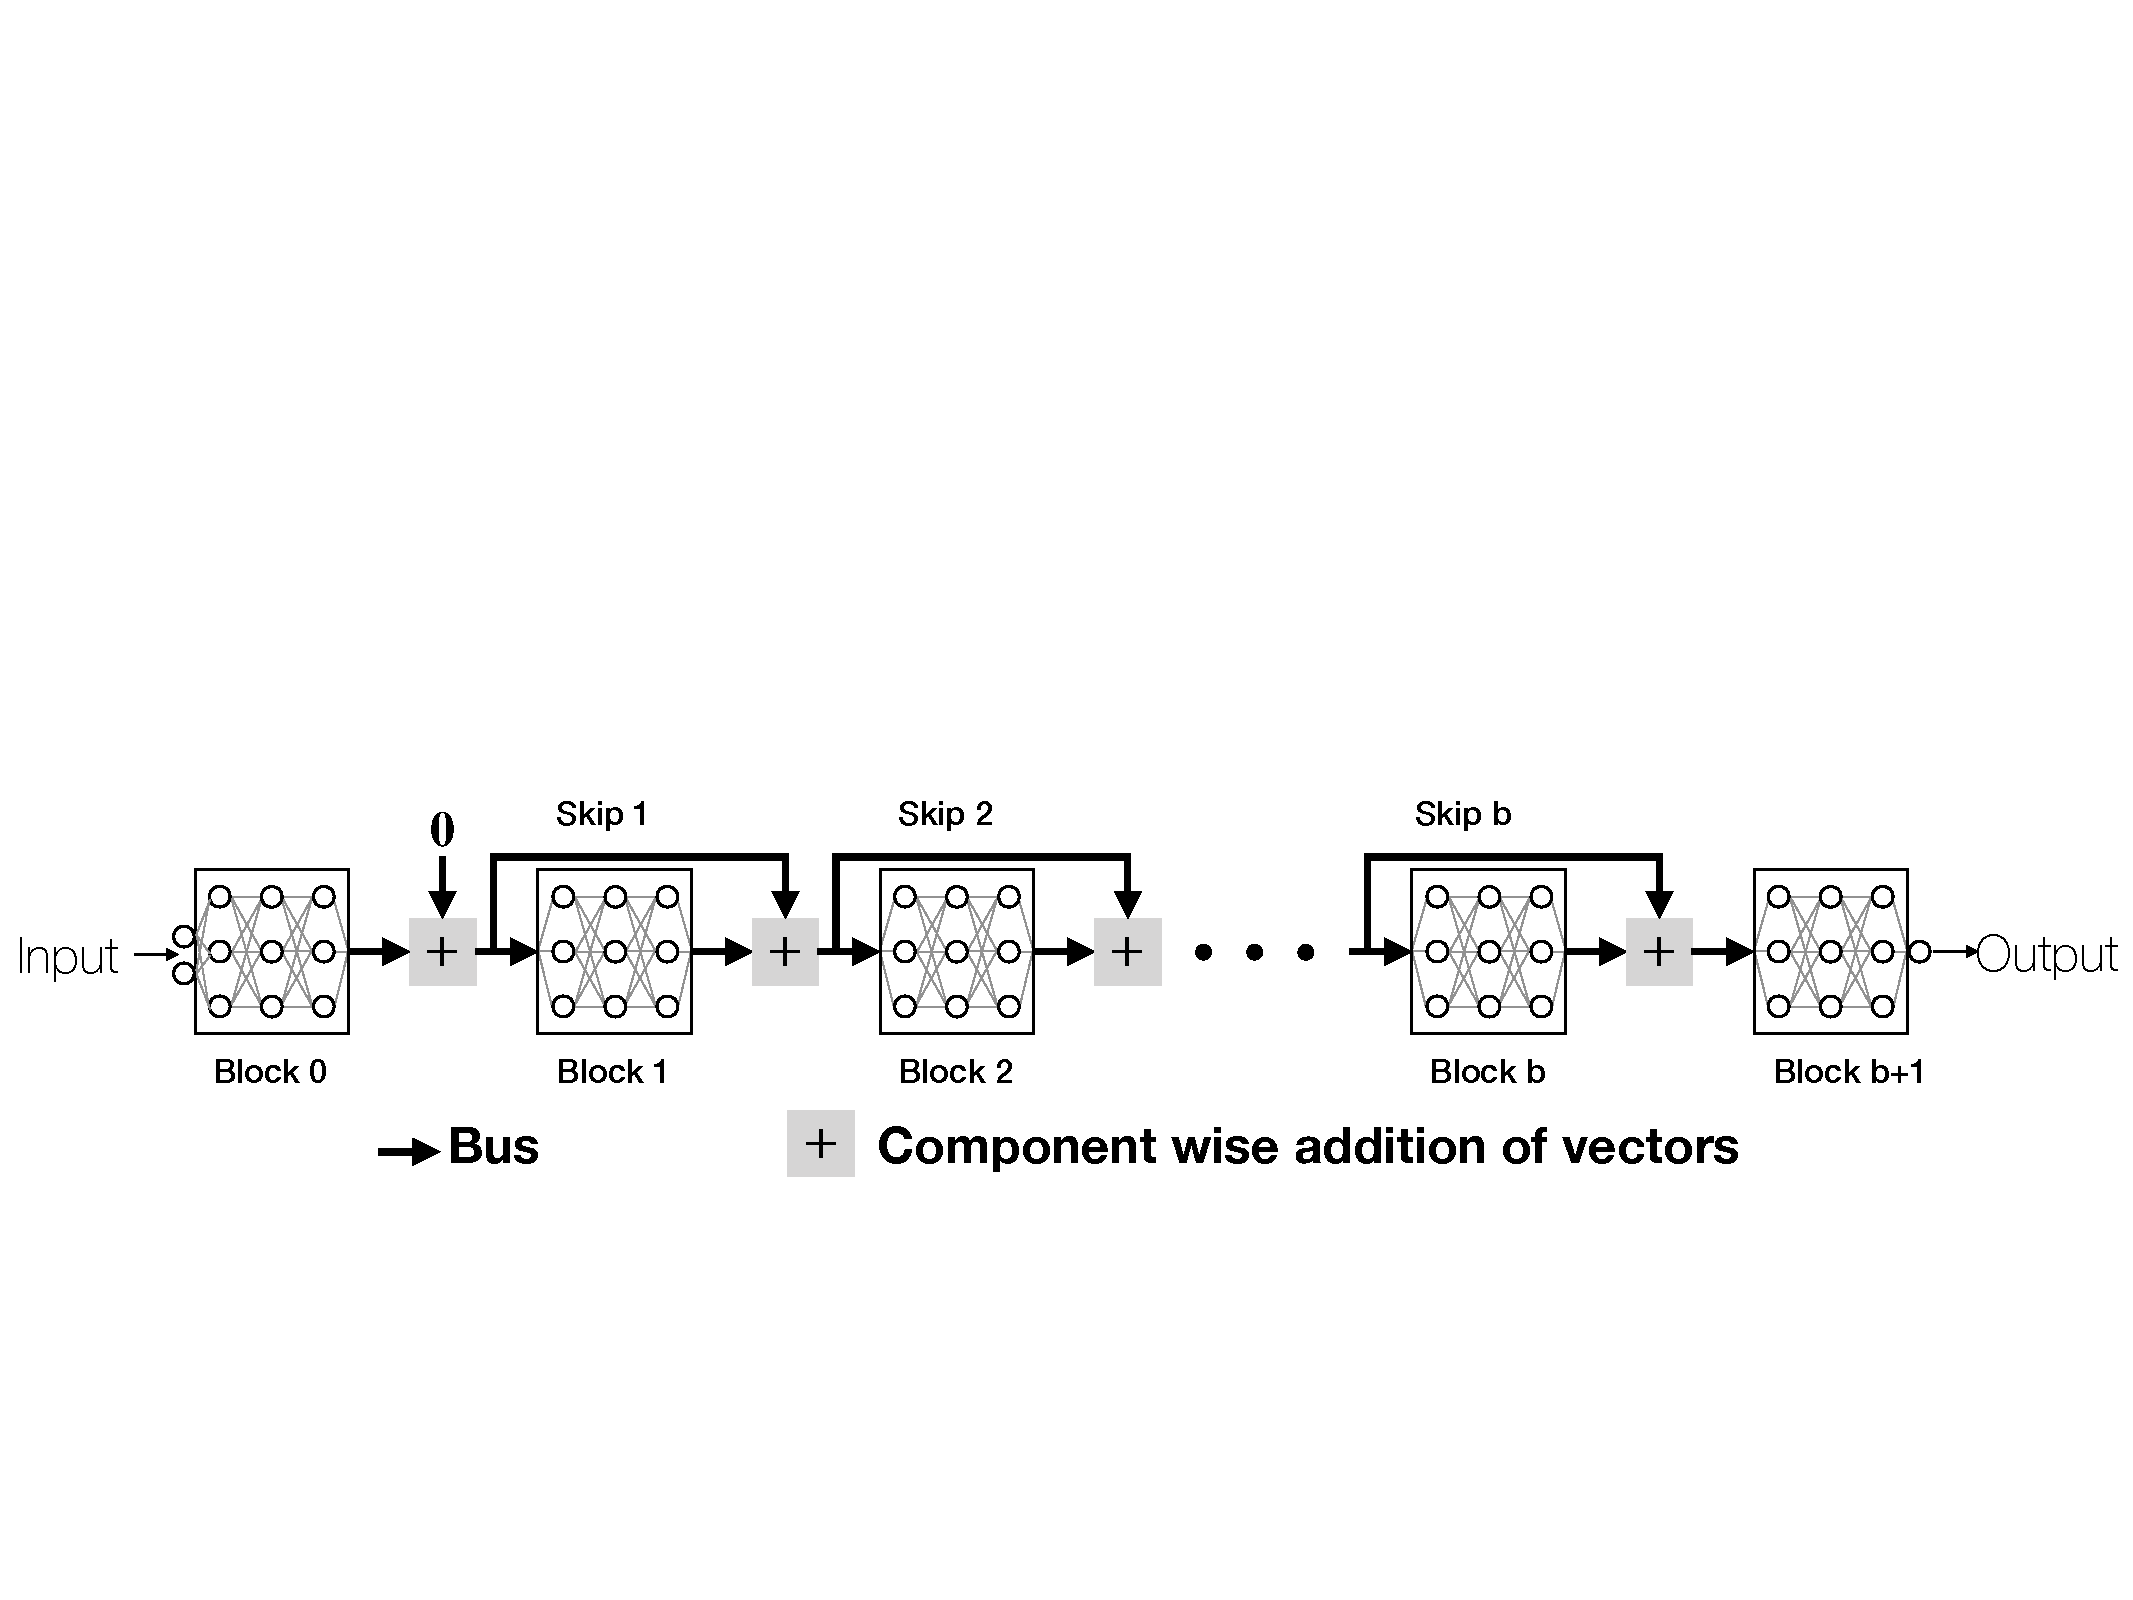
\includegraphics[scale=0.5]{figs/resnet.pdf}
}
\caption{\small{ResNet with $b$ skip connections and $(b+2)$ blocks.}}
\label{fig:resnet}
\end{figure}
\begin{definition}\label{def:subfcdnn}[Sub FC-DNNs]
Let $2^{[b]}$ denote the power set of $[b]$ and let $\J\in 2^{[b]}$ denote any subset of $[b]$. Define the`$\J^{th}$' sub-FC-DNN of the ResNet to be the fully connected network obtained by (i) ignoring/removing (see \Cref{fig:resnet}) the skip connections $\text{skip}_j,\forall j\in \J$ (see \Cref{fig:resnet}), and (ii) ignoring $\text{block}_{j},\forall j\in \J$.
\end{definition}
%\Cref{fig:subfcdnn} shows the $4$ sub-FC-DNNs namely $H^i,i=1,2,3,4$ in the case of $b=2$ skip connections.
\FloatBarrier
\begin{figure}[h]
\resizebox{\columnwidth}{!}{
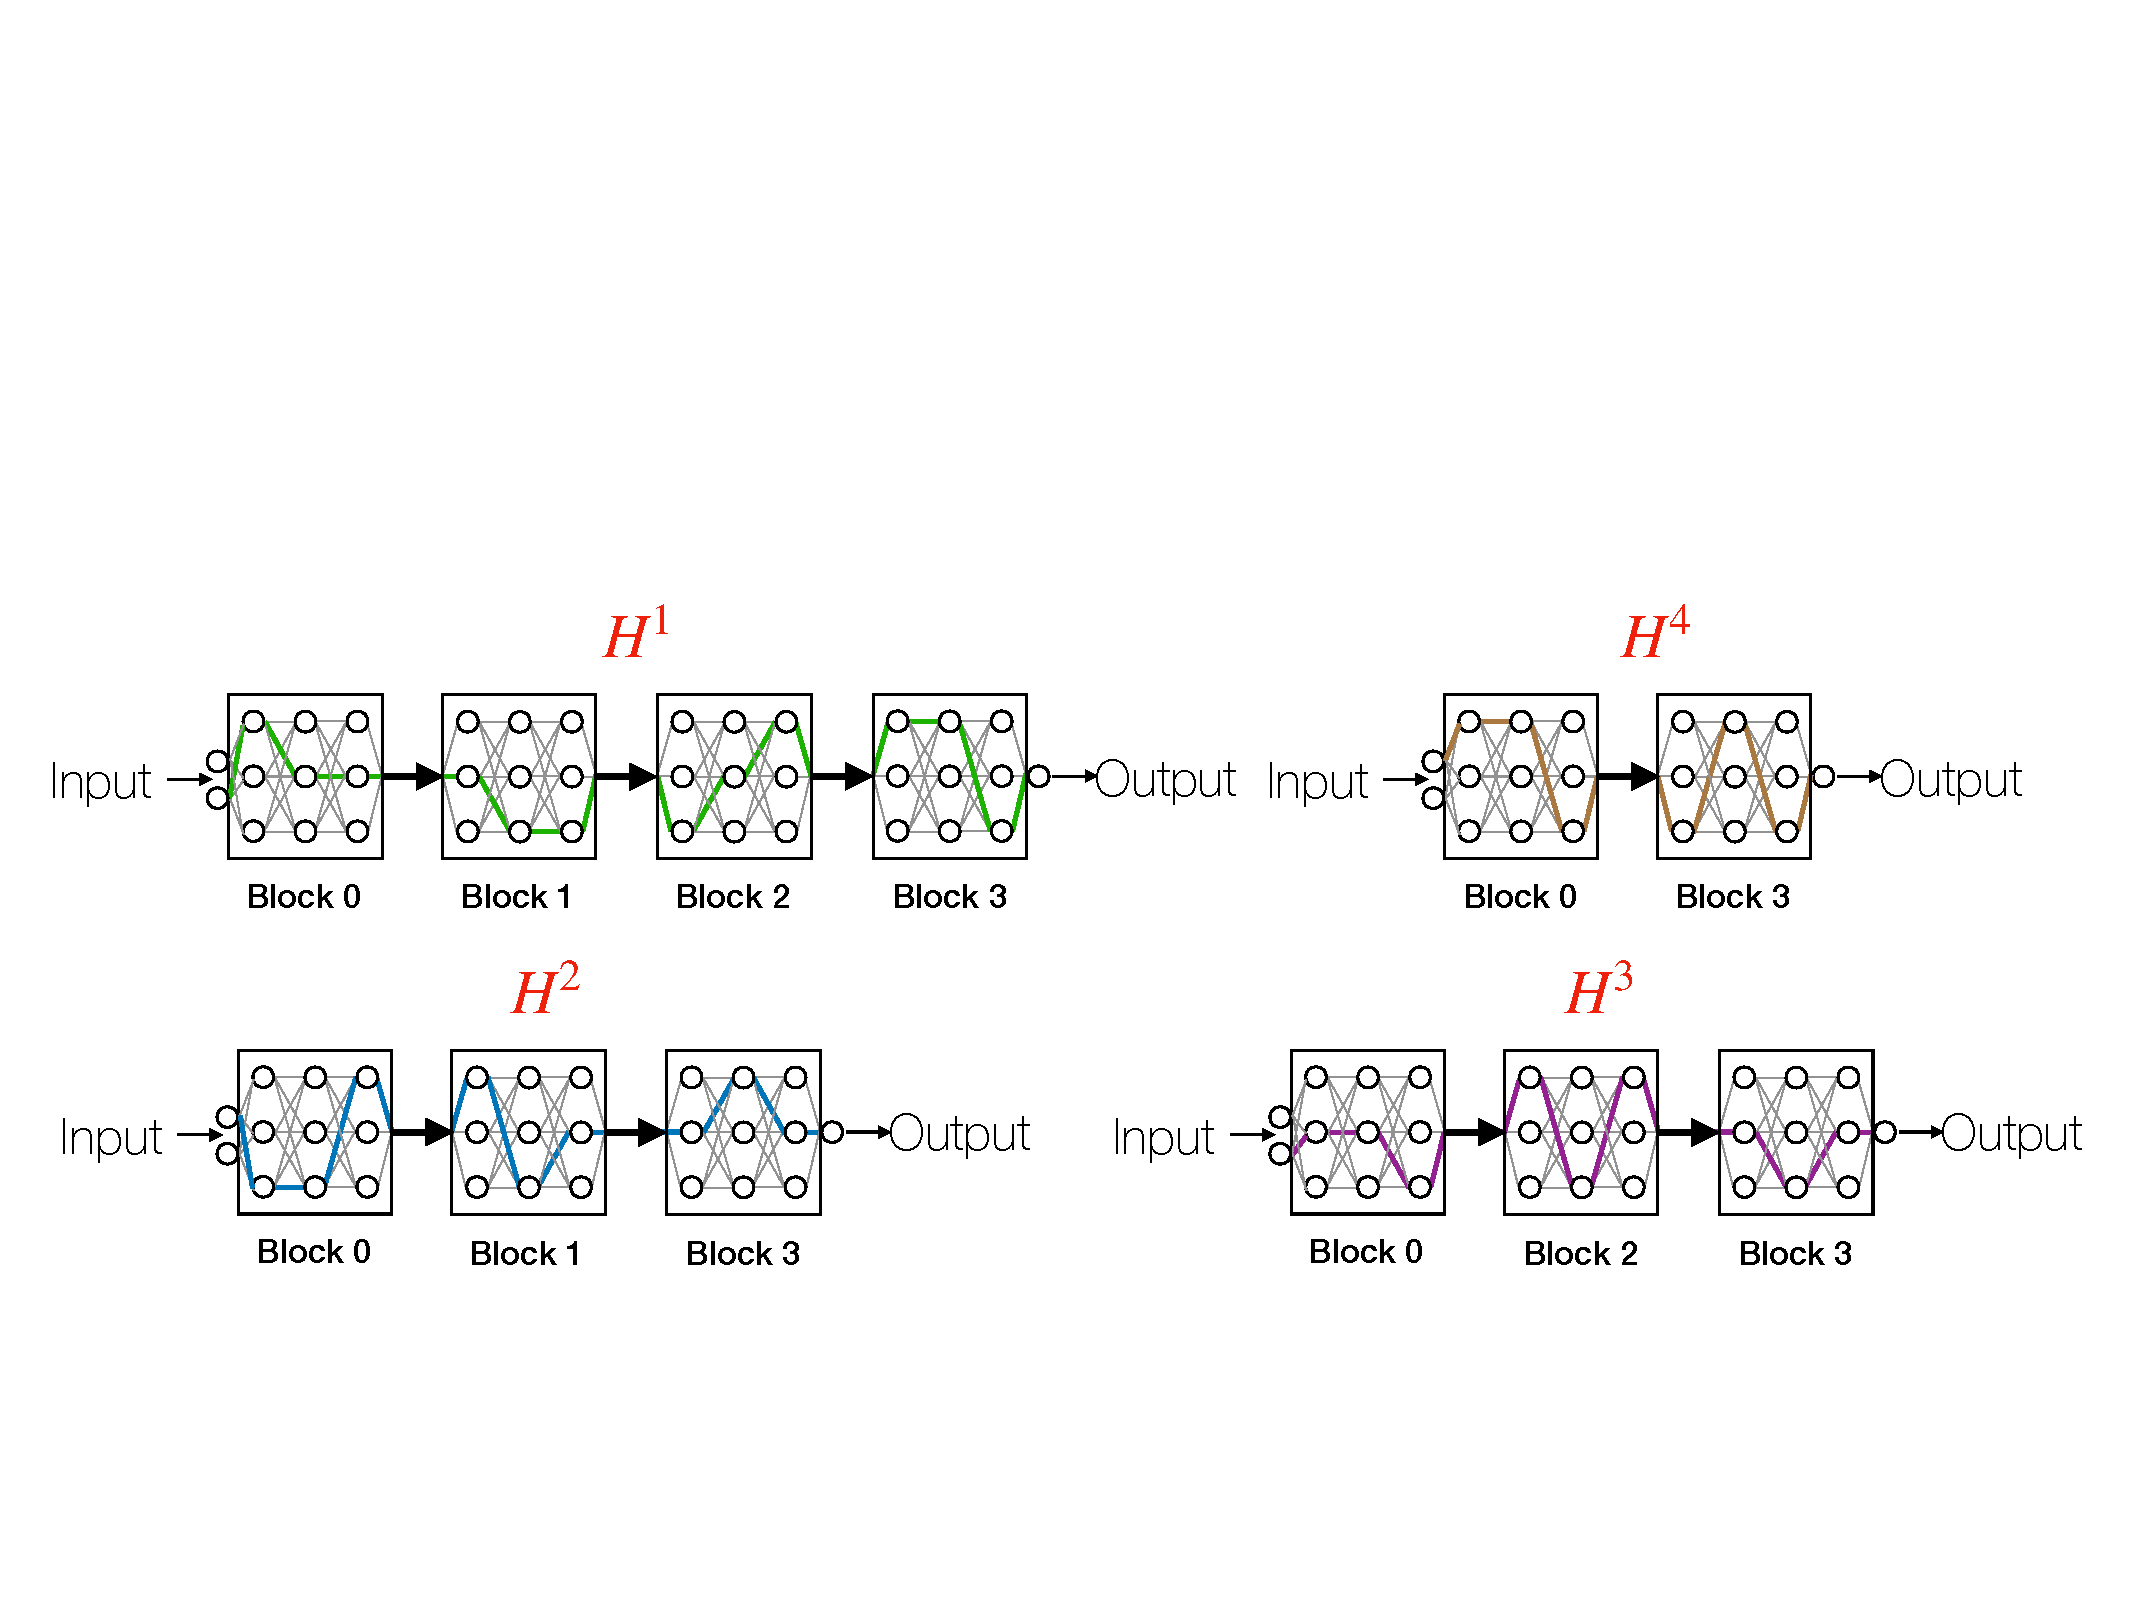
\includegraphics[scale=0.5]{figs/blocks.pdf}
}
\caption{\small{$H^i,i\in[4]$ are the $2^2$ sub-FC-DNNs in a ResNet with $b=2$. Thicker lines in $H^i,i\in[4]$ denote paths. Different grey levels indicate that for $i\neq j$ paths of $H^i$ and $H^j$ are distinct.}}
\label{fig:subfcdnn}
\end{figure}
\begin{comment}
\begin{notation}[Index Maps]
Let $\I^{\J}(p)\colon [\Pres]\ra 2^{[b]}$ specify the indices of the skip connections ignored in path $p$.  Also, we follow the convention that weights and gating values of layers corresponding to blocks skipped are $1$.
\end{notation}
\end{comment}
\begin{lemma}[Sum of Product Kernel]\label{lm:sumofproduct}
Let $H^{\text{res}}_{\Theta}$ be the NPK of the ResNet, and $H^{\J}_{\Theta}$ be the NPK of the sub-FC-DNN within the ResNet obtained by ignoring those skip connections in the set $\J$. Then, \begin{align*}H^{\text{res}}_{\Theta}=\sum_{\J\in 2^{[b]}}H^{\J}_{\Theta}\end{align*}
%\begin{align*}
%\end{align*}
\end{lemma}

\begin{theorem}\label{th:mainres} Let $\sigma=\frac{\cscale}{\sqrt{w}}$. Under \Cref{assmp:main}, as $w\ra\infty$,  for $\bres^{\J} = (|\J| +2)\cdot\dblock\cdot \sigfc^{2\big( (|\J|+2)\dblock-1\big)}$,
\begin{align*}
\kv_{\Tdgn_0}\ra \sum_{\J\in 2^{[b]}}  \bres^{\J} H^{\J}_{\Tf_0}
\end{align*}
\end{theorem}
